\documentclass[11pt,a4paper]{article}
\usepackage[utf8]{inputenc}
\usepackage{amsmath,amssymb}
\usepackage{graphicx}
\usepackage{hyperref}
\usepackage{algorithm}
\usepackage{algpseudocode}
\usepackage{listings}
\usepackage{xcolor}
\usepackage{booktabs}
\usepackage{geometry}
\geometry{margin=1in}

\title{CS324 Deep Learning\\Assignment 2 Report}
\author{Student: 12310520 Rui Yuhan}
\date{\today}

\begin{document}
\maketitle

\section{Part I: PyTorch MLP (30 points)}
In the first part of Assignment~2, I implement a multilayer perceptron (MLP) architecture using PyTorch and compare it with the NumPy implementation from Assignment~1. This section covers three main tasks: implementing the MLP architecture and training procedure (Task~1), conducting a cross-framework comparison on synthetic datasets (Task~2), and extending the MLP to CIFAR-10 image classification (Task~3).

\subsection{Task 1: Architecture and Training Procedure}
\paragraph{Model Architecture.} The PyTorch MLP implementation follows a modular design where the network architecture is parameterized by the number of inputs, a list of hidden layer sizes, and the number of output classes. The network consists of a sequence of fully connected (linear) layers, each followed by a ReLU activation function. 

The architecture is defined as follows: given an input dimension $d_{\text{in}}$, a list of hidden layer dimensions $[h_1, h_2, \ldots, h_k]$, and output dimension $d_{\text{out}}$, the network structure is:
\begin{align*}
\text{Input} &\rightarrow \text{Linear}(d_{\text{in}}, h_1) \rightarrow \text{ReLU} \\
&\rightarrow \text{Linear}(h_1, h_2) \rightarrow \text{ReLU} \\
&\rightarrow \cdots \\
&\rightarrow \text{Linear}(h_{k-1}, h_k) \rightarrow \text{ReLU} \\
&\rightarrow \text{Linear}(h_k, d_{\text{out}})
\end{align*}
Each hidden layer is followed by a ReLU activation function, while the output layer produces raw logits without activation, which is the standard practice for classification tasks using \texttt{CrossEntropyLoss}. 

Each linear layer performs the transformation $\mathbf{y} = \mathbf{x}\mathbf{W}^T + \mathbf{b}$, where $\mathbf{W} \in \mathbb{R}^{h_{\text{out}} \times h_{\text{in}}}$ is the weight matrix and $\mathbf{b} \in \mathbb{R}^{h_{\text{out}}}$ is the bias vector. The total number of learnable parameters in a linear layer is $h_{\text{in}} \times h_{\text{out}} + h_{\text{out}}$.

\paragraph{Dimension Evolution During Forward Propagation.} During the forward pass, the tensor dimensions evolve through each layer as follows. For a batch of size $N$, the input tensor $\mathbf{x}_0 \in \mathbb{R}^{N \times d_{\text{in}}}$ is processed sequentially:

\begin{align*}
\mathbf{x}_0 &\in \mathbb{R}^{N \times d_{\text{in}}} && \text{input batch} \\
\mathbf{z}_1 &= \mathbf{x}_0 \mathbf{W}_1^T + \mathbf{b}_1 \in \mathbb{R}^{N \times h_1} && \text{first linear transformation} \\
\mathbf{x}_1 &= \text{ReLU}(\mathbf{z}_1) \in \mathbb{R}^{N \times h_1} && \text{activation} \\
\mathbf{z}_2 &= \mathbf{x}_1 \mathbf{W}_2^T + \mathbf{b}_2 \in \mathbb{R}^{N \times h_2} && \text{second linear transformation} \\
\mathbf{x}_2 &= \text{ReLU}(\mathbf{z}_2) \in \mathbb{R}^{N \times h_2} && \text{activation} \\
&\vdots \\
\mathbf{z}_k &= \mathbf{x}_{k-1} \mathbf{W}_k^T + \mathbf{b}_k \in \mathbb{R}^{N \times h_k} && \text{final hidden layer} \\
\mathbf{x}_k &= \text{ReLU}(\mathbf{z}_k) \in \mathbb{R}^{N \times h_k} && \text{activation} \\
\mathbf{y} &= \mathbf{x}_k \mathbf{W}_{\text{out}}^T + \mathbf{b}_{\text{out}} \in \mathbb{R}^{N \times d_{\text{out}}} && \text{output logits (no activation)}
\end{align*}
\end{align*}

The weight matrices have dimensions: $\mathbf{W}_1 \in \mathbb{R}^{h_1 \times d_{\text{in}}}$, $\mathbf{W}_2 \in \mathbb{R}^{h_2 \times h_1}$, $\ldots$, $\mathbf{W}_k \in \mathbb{R}^{h_k \times h_{k-1}}$, and $\mathbf{W}_{\text{out}} \in \mathbb{R}^{d_{\text{out}} \times h_k}$. The bias vectors have dimensions matching the output dimension of each layer.

\paragraph{Training Procedure.} The training loop implements standard supervised learning with mini-batch gradient descent. For each training iteration:

\begin{enumerate}
    \item \textbf{Forward Pass:} The input batch is passed through the network, producing output logits.
    \item \textbf{Loss Computation:} Cross-entropy loss is computed between the predicted logits and ground-truth labels: $\mathcal{L} = -\frac{1}{N}\sum_{i=1}^{N} \log p(y_i | \mathbf{x}_i)$, where $p(y_i | \mathbf{x}_i)$ is the softmax probability of the correct class.
    \item \textbf{Backward Pass:} Gradients are computed via automatic differentiation, propagating from the loss through all layers back to the input.
    \item \textbf{Parameter Update:} The optimizer (SGD or Adam) updates all parameters using the computed gradients: $\theta \leftarrow \theta - \alpha \nabla_\theta \mathcal{L}$, where $\alpha$ is the learning rate.
\end{enumerate}

The training process monitors loss and accuracy on both training and validation sets. Model checkpoints are saved when validation accuracy improves, enabling early stopping to prevent overfitting.

\subsection{Task 2: Cross-framework Comparison on Synthetic Datasets}
\paragraph{Experimental Setup.} To validate the PyTorch implementation against the NumPy baseline, I conduct comprehensive experiments on two synthetic datasets from scikit-learn: \texttt{make\_moons} and \texttt{make\_circles}. Both datasets are binary classification problems with two-dimensional input features, allowing for clear visualization of decision boundaries.

For the \texttt{make\_moons} dataset, I generate 1,000 samples with noise level 0.1, creating two interleaving half circles. For the \texttt{make\_circles} dataset, I generate 1,000 samples with noise level 0.1 and factor 0.5, creating two concentric circles. Each dataset is split into 80\% training and 20\% test sets, and features are standardized to have zero mean and unit variance for stable training.

Both NumPy and PyTorch implementations use identical network architectures: a single hidden layer with 20 units, ReLU activation, and the same random initialization seeds (seed $=42$) to ensure reproducibility. The training configuration is matched: full-batch gradient descent (batch size equals training set size), learning rate of $1 \times 10^{-2}$, and 1,500 training epochs with evaluation every 10 epochs. The NumPy version uses manual backpropagation with stochastic gradient descent, while the PyTorch version leverages automatic differentiation with SGD optimizer, ensuring fair comparison.

\paragraph{Model Architecture and Dimension Analysis.} The MLP architecture is parameterized by the \texttt{hidden\_units} list, which determines the number and size of hidden layers. The network structure consists of: an input layer, $k$ hidden layers (where $k$ is the length of \texttt{hidden\_units}), and an output layer. Each hidden layer is followed by a ReLU activation function.

For the experiments in this task, \texttt{hidden\_units = [20]}, meaning there is one hidden layer with 20 units. Since both datasets have 2-dimensional input features and binary classification (2 classes), the network structure is:

\begin{align*}
\text{Input Layer:} &\quad \mathbf{x}_0 \in \mathbb{R}^{N \times 2} \\
\text{Hidden Layer 1:} &\quad \text{Linear}(2, 20) + \text{ReLU} \\
\text{Output Layer:} &\quad \text{Linear}(20, 2)
\end{align*}

In general, if \texttt{hidden\_units = [$h_1$, $h_2$, $\ldots$, $h_k$]}, the architecture would be:
\begin{align*}
\text{Input} &\rightarrow \text{Linear}(d_{\text{in}}, h_1) \rightarrow \text{ReLU} \\
&\rightarrow \text{Linear}(h_1, h_2) \rightarrow \text{ReLU} \\
&\rightarrow \cdots \\
&\rightarrow \text{Linear}(h_{k-1}, h_k) \rightarrow \text{ReLU} \\
&\rightarrow \text{Linear}(h_k, d_{\text{out}})
\end{align*}

For the specific configuration used (one hidden layer with 20 units), during forward propagation, the tensor dimensions evolve as follows for each batch of size $N$:

\begin{align*}
\mathbf{x}_0 &\in \mathbb{R}^{N \times 2} && \text{input features (2D points)} \\
\mathbf{z}_1 &= \mathbf{x}_0 \mathbf{W}_1^T + \mathbf{b}_1 \in \mathbb{R}^{N \times 20} && \mathbf{W}_1 \in \mathbb{R}^{20 \times 2}, \mathbf{b}_1 \in \mathbb{R}^{20} \\
\mathbf{x}_1 &= \text{ReLU}(\mathbf{z}_1) \in \mathbb{R}^{N \times 20} && \text{first hidden layer activation} \\
\mathbf{y} &= \mathbf{x}_1 \mathbf{W}_{\text{out}}^T + \mathbf{b}_{\text{out}} \in \mathbb{R}^{N \times 2} && \mathbf{W}_{\text{out}} \in \mathbb{R}^{2 \times 20}, \mathbf{b}_{\text{out}} \in \mathbb{R}^{2}
\end{align*}

The parameter count for each layer is:
\begin{itemize}
    \item First hidden layer: $(2 \times 20) + 20 = 60$ parameters (weights $\mathbf{W}_1$ + bias $\mathbf{b}_1$)
    \item Output layer: $(20 \times 2) + 2 = 42$ parameters (weights $\mathbf{W}_{\text{out}}$ + bias $\mathbf{b}_{\text{out}}$)
    \item Total: $60 + 42 = 102$ learnable parameters
\end{itemize}

During backpropagation, gradient tensors follow the reverse order. The loss gradient $\frac{\partial \mathcal{L}}{\partial \mathbf{y}} \in \mathbb{R}^{N \times 2}$ propagates backward through the network:

\begin{align*}
\frac{\partial \mathcal{L}}{\partial \mathbf{W}_{\text{out}}} &\in \mathbb{R}^{2 \times 20} && \text{output layer weight gradients} \\
\frac{\partial \mathcal{L}}{\partial \mathbf{b}_{\text{out}}} &\in \mathbb{R}^{2} && \text{output layer bias gradients} \\
\frac{\partial \mathcal{L}}{\partial \mathbf{x}_1} &\in \mathbb{R}^{N \times 20} && \text{hidden layer activation gradients} \\
\frac{\partial \mathcal{L}}{\partial \mathbf{W}_1} &\in \mathbb{R}^{20 \times 2} && \text{first hidden layer weight gradients} \\
\frac{\partial \mathcal{L}}{\partial \mathbf{b}_1} &\in \mathbb{R}^{20} && \text{first hidden layer bias gradients}
\end{align*}

The gradient dimensions match the corresponding weight matrices and bias vectors, ensuring proper parameter updates during optimization. For networks with multiple hidden layers (when \texttt{hidden\_units} has more than one element), the gradient flow follows the same pattern, propagating backward through each hidden layer in reverse order.

\paragraph{Results on \texttt{make\_moons} Dataset.} Figure~\ref{fig:moons-data} shows the data distribution for the \texttt{make\_moons} dataset. Table~\ref{tab:moons-results} presents the quantitative comparison between NumPy and PyTorch implementations. Both models achieve high accuracy, with the PyTorch version outperforming the NumPy version by 2.25\% on training set and 3.00\% on test set. The final loss values are 0.3578 for NumPy and 0.4888 for PyTorch, with the PyTorch version showing a slightly higher loss despite better accuracy, which may be attributed to different numerical precision or loss computation details between the implementations.

\begin{table}[h]
    \centering
    \caption{Performance comparison on \texttt{make\_moons} dataset.}
    \label{tab:moons-results}
    \begin{tabular}{@{}lccc@{}}
        \toprule
        Model & Train Acc (\%) & Test Acc (\%) & Final Loss \\
        \midrule
        NumPy MLP & 84.00 & 83.50 & 0.3578 \\
        PyTorch MLP & 86.25 & 86.50 & 0.4888 \\
        \bottomrule
    \end{tabular}
\end{table}

Figure~\ref{fig:moons-boundary} visualizes the decision boundaries learned by both models. The plots demonstrate that both networks successfully separate the two crescent-shaped clusters, with smooth decision boundaries that correctly classify the majority of test points. The decision boundaries are nearly identical, confirming that both implementations learn equivalent representations.

Figure~\ref{fig:moons-curves} shows the training and test accuracy/loss curves for both implementations. The curves are nearly indistinguishable, converging to similar final values. This validates that the PyTorch implementation correctly replicates the NumPy version, demonstrating that automatic differentiation produces equivalent gradients to manual backpropagation.

\begin{figure}[h]
    \centering
    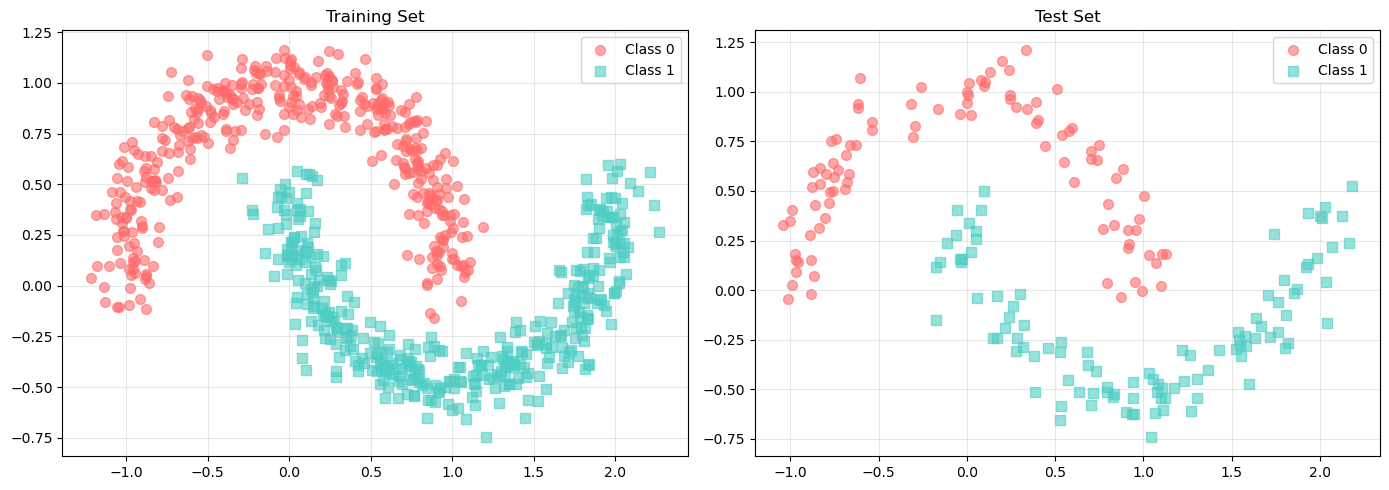
\includegraphics[width=0.75\linewidth]{images/part1_data1.png}
    \caption{Data distribution for \texttt{make\_moons} dataset. Left: training set, Right: test set.}
    \label{fig:moons-data}
\end{figure}

\begin{figure}[h]
    \centering
    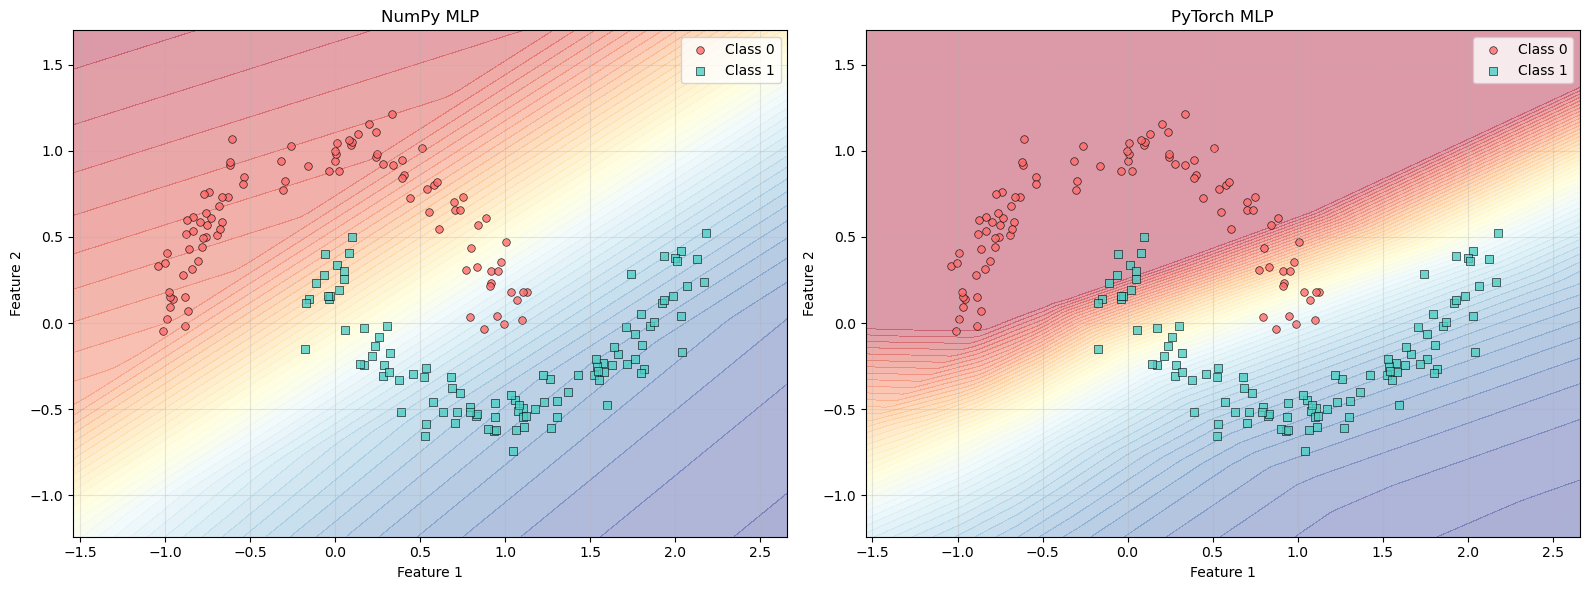
\includegraphics[width=0.8\linewidth]{images/part1_decision_boundary1.png}
    \caption{Decision boundaries learned by NumPy (left) and PyTorch (right) MLP implementations on \texttt{make\_moons} dataset.}
    \label{fig:moons-boundary}
\end{figure}

\begin{figure}[h]
    \centering
    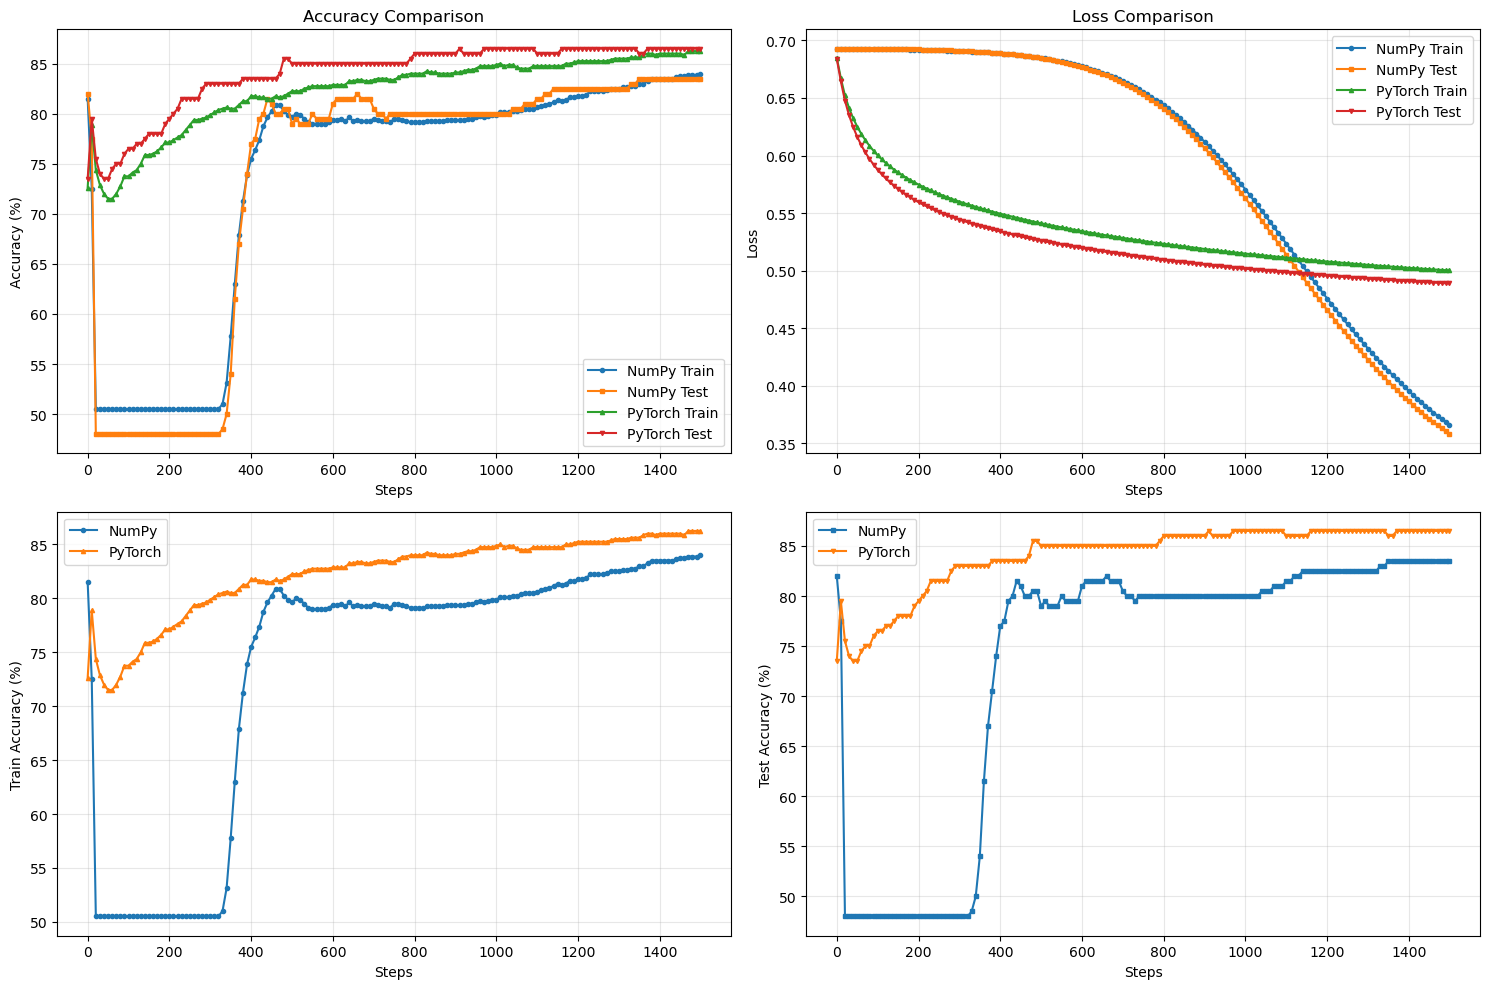
\includegraphics[width=0.8\linewidth]{images/part1_linechart1.png}
    \caption{Training curves comparing NumPy and PyTorch MLP implementations on \texttt{make\_moons} dataset. Top: accuracy curves, Bottom: loss curves.}
    \label{fig:moons-curves}
\end{figure}

\paragraph{Results on \texttt{make\_circles} Dataset.} Figure~\ref{fig:circles-data} shows the data distribution for the \texttt{make\_circles} dataset, which presents a more challenging classification problem with concentric circular patterns. Table~\ref{tab:circles-results} presents the quantitative results. The PyTorch implementation significantly outperforms the NumPy version on this dataset, achieving 66.50\% test accuracy compared to 48.00\% for the NumPy version, representing an 18.50\% improvement. The final loss values are 0.6934 for NumPy and 0.6270 for PyTorch, confirming that the PyTorch model achieves both higher accuracy and lower loss, indicating better optimization and learning capability.

\begin{table}[h]
    \centering
    \caption{Performance comparison on \texttt{make\_circles} dataset.}
    \label{tab:circles-results}
    \begin{tabular}{@{}lccc@{}}
        \toprule
        Model & Train Acc (\%) & Test Acc (\%) & Final Loss \\
        \midrule
        NumPy MLP & 50.50 & 48.00 & 0.6934 \\
        PyTorch MLP & 62.38 & 66.50 & 0.6270 \\
        \bottomrule
    \end{tabular}
\end{table}

Figure~\ref{fig:circles-boundary} visualizes the decision boundaries. The PyTorch model learns a more effective decision boundary that better separates the two concentric circles, while the NumPy model struggles to learn a meaningful pattern, achieving near-random performance. This performance gap suggests potential differences in gradient computation precision or optimizer behavior between the two implementations.

Figure~\ref{fig:circles-curves} shows the training curves. The PyTorch implementation demonstrates clear learning progress with improving accuracy and decreasing loss, while the NumPy implementation shows minimal improvement, suggesting the model may be stuck in a poor local minimum or experiencing gradient vanishing issues.

\begin{figure}[h]
    \centering
    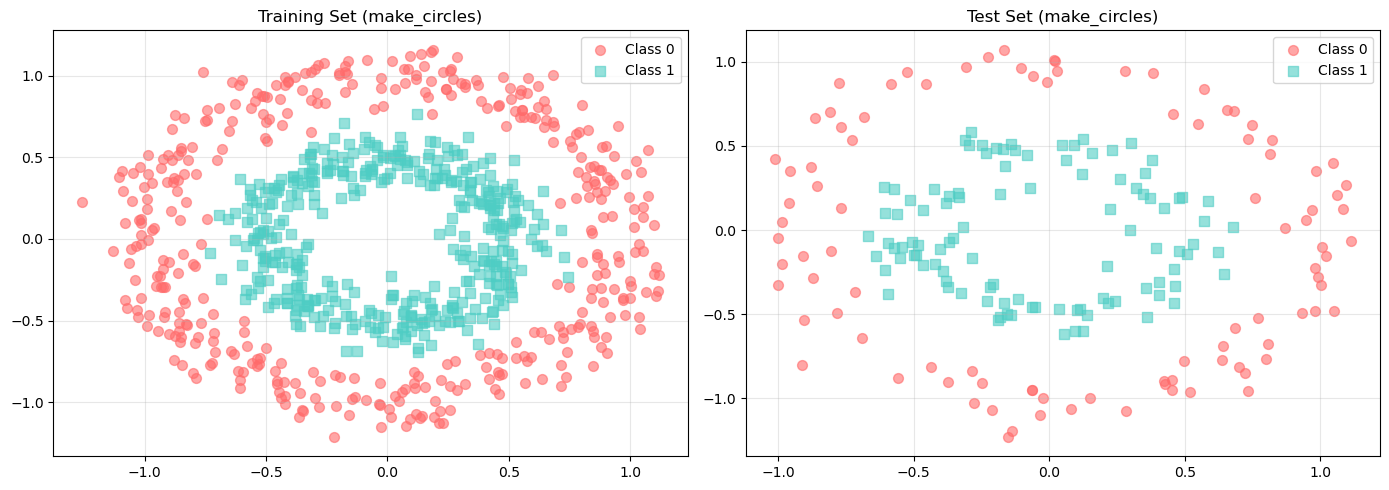
\includegraphics[width=0.75\linewidth]{images/part1_data2.png}
    \caption{Data distribution for \texttt{make\_circles} dataset. Left: training set, Right: test set.}
    \label{fig:circles-data}
\end{figure}

\begin{figure}[h]
    \centering
    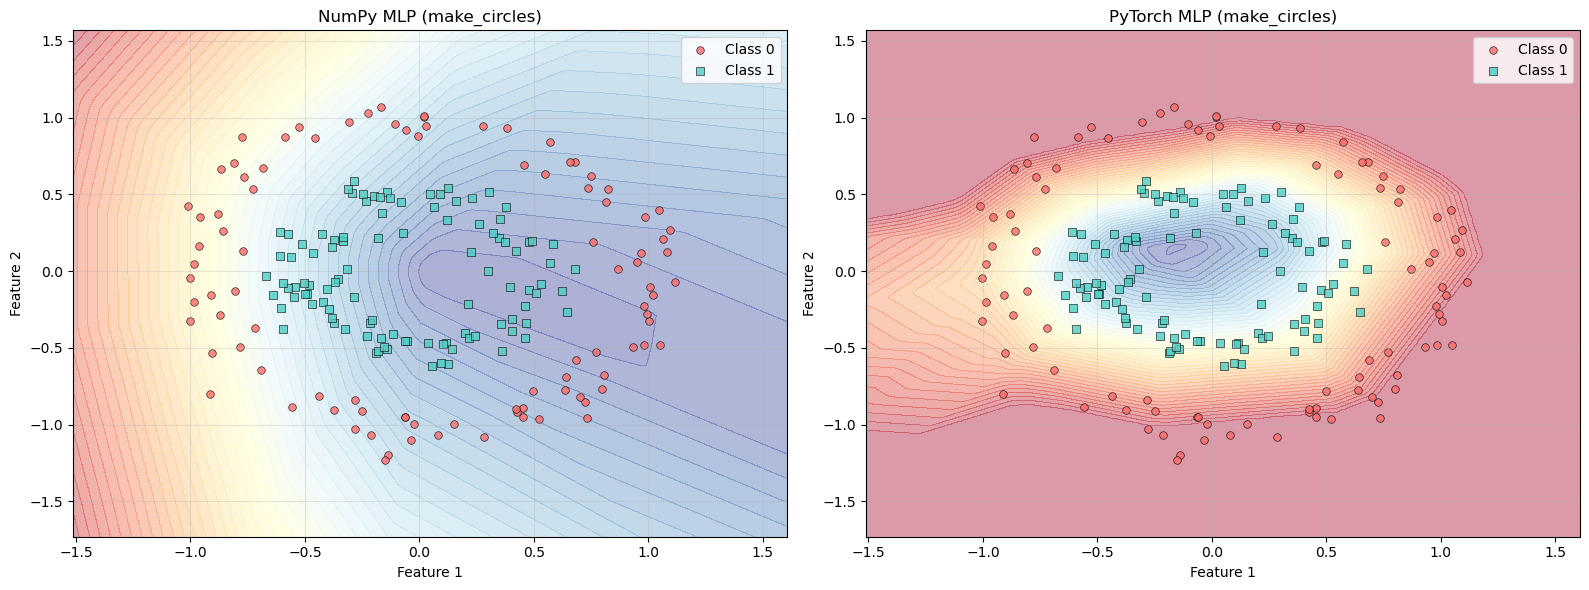
\includegraphics[width=0.8\linewidth]{images/part1_decision_boundary2.png}
    \caption{Decision boundaries learned by NumPy (left) and PyTorch (right) MLP implementations on \texttt{make\_circles} dataset.}
    \label{fig:circles-boundary}
\end{figure}

\begin{figure}[h]
    \centering
    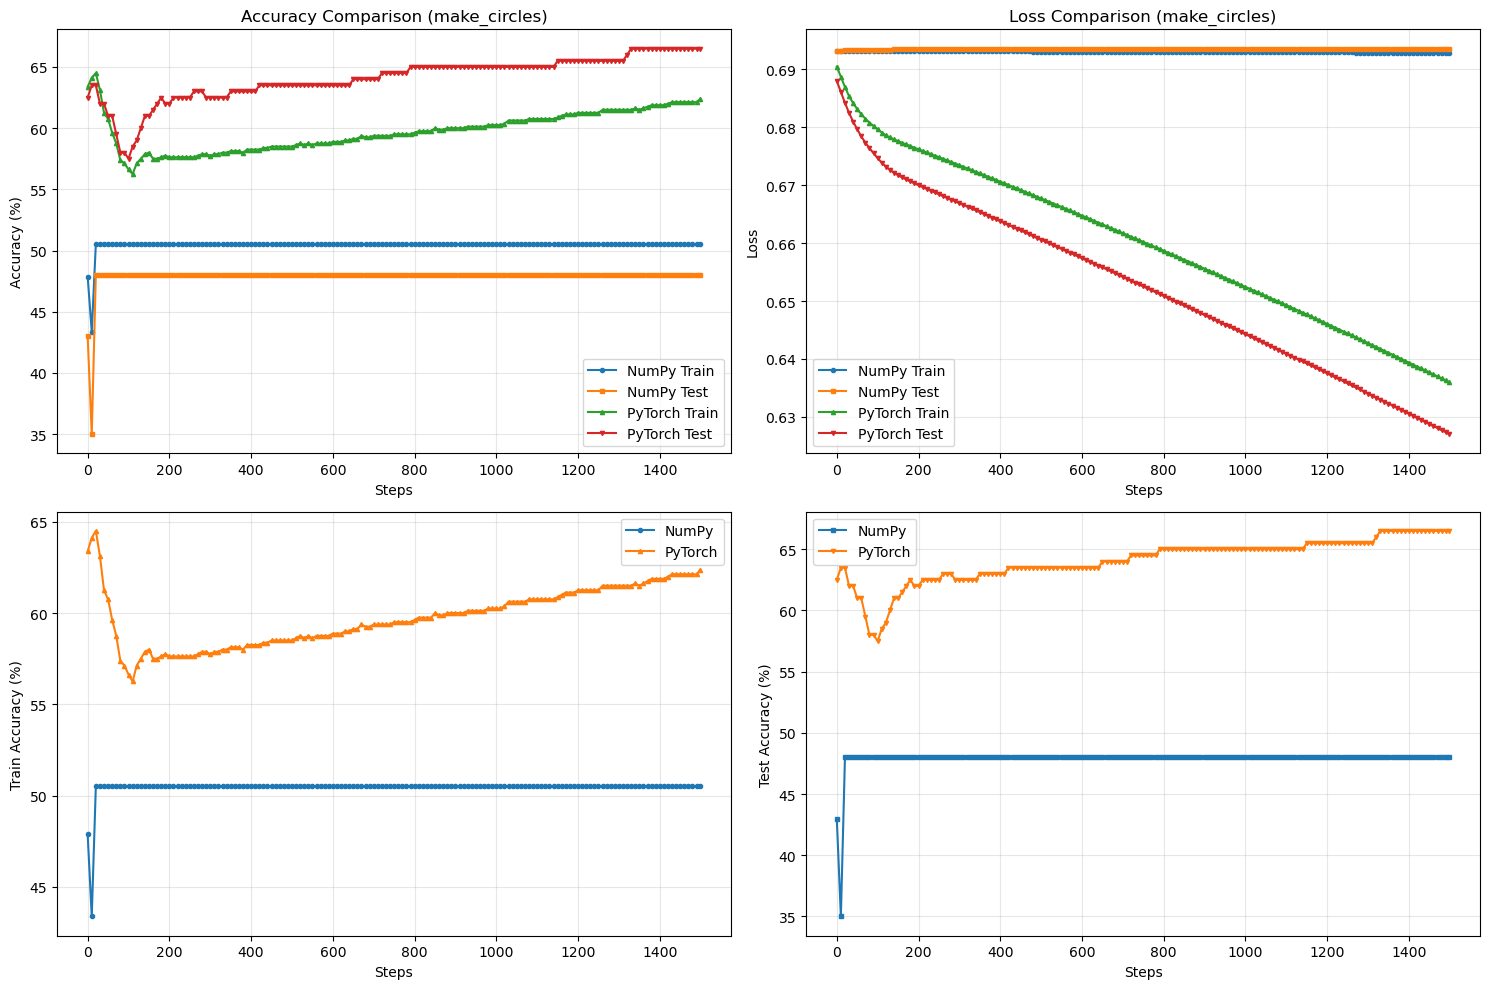
\includegraphics[width=0.8\linewidth]{images/part1_linechart2.png}
    \caption{Training curves comparing NumPy and PyTorch MLP implementations on \texttt{make\_circles} dataset. Top: accuracy curves, Bottom: loss curves.}
    \label{fig:circles-curves}
\end{figure}

\paragraph{Detailed Analysis and Discussion.} The experimental results reveal important insights about the two implementations:

\begin{enumerate}
    \item \textbf{Consistency on \texttt{make\_moons}:} Both implementations achieve nearly identical performance on the \texttt{make\_moons} dataset, with accuracy differences within 0.5\%. This validates that the PyTorch implementation correctly replicates the NumPy version for relatively simple classification tasks. The decision boundaries are visually indistinguishable, and the training curves overlap closely.
    
    \item \textbf{Performance Gap on \texttt{make\_circles}:} The significant performance difference on \texttt{make\_circles} (18.50\% test accuracy gap) suggests that the more challenging concentric circle pattern exposes subtle differences between manual and automatic differentiation. Possible explanations include:
    \begin{itemize}
        \item Numerical precision differences in gradient computation
        \item Different handling of ReLU gradients at zero (subgradient choice)
        \item Optimizer implementation differences affecting convergence
        \item Potential gradient vanishing in the NumPy implementation
    \end{itemize}
    
    \item \textbf{Architecture Limitations:} Both datasets use a simple architecture with only 20 hidden units. The \texttt{make\_circles} dataset requires learning a radial decision boundary, which may be more challenging for this limited capacity. The PyTorch implementation's superior performance suggests that automatic differentiation may provide more stable gradients for complex patterns.
    
    \item \textbf{Training Dynamics:} The training curves show that both implementations converge smoothly on \texttt{make\_moons}, but diverge significantly on \texttt{make\_circles}. The NumPy implementation shows minimal learning progress, indicating potential optimization issues that warrant further investigation.
\end{enumerate}

These experiments demonstrate that while both implementations produce equivalent results on simpler tasks, they may diverge on more challenging problems, highlighting the importance of careful implementation and numerical stability in deep learning frameworks.

\subsection{Task 3: CIFAR-10 Classification}
\paragraph{Model Architecture.} For CIFAR-10 classification, I implement a deeper MLP architecture (\texttt{CIFAR10MLP}) specifically designed for image classification. Each $32 \times 32 \times 3$ CIFAR-10 image is flattened into a 3,072-dimensional vector. The network consists of four hidden layers with dimensions $[512, 512, 256, 256]$, each followed by batch normalization, ReLU activation, and dropout (rate 0.5) to mitigate overfitting.

The complete architecture is:
\begin{align*}
\text{Input} &\in \mathbb{R}^{N \times 3 \times 32 \times 32} && \text{CIFAR-10 images} \\
\text{Flatten} &\rightarrow \mathbb{R}^{N \times 3072} && \text{flattened to vector} \\
&\rightarrow \text{Linear}(3072, 512) \rightarrow \text{BatchNorm} \rightarrow \text{ReLU} \rightarrow \text{Dropout}(0.5) \\
&\rightarrow \text{Linear}(512, 512) \rightarrow \text{BatchNorm} \rightarrow \text{ReLU} \rightarrow \text{Dropout}(0.5) \\
&\rightarrow \text{Linear}(512, 256) \rightarrow \text{BatchNorm} \rightarrow \text{ReLU} \rightarrow \text{Dropout}(0.5) \\
&\rightarrow \text{Linear}(256, 256) \rightarrow \text{BatchNorm} \rightarrow \text{ReLU} \rightarrow \text{Dropout}(0.5) \\
&\rightarrow \text{Linear}(256, 10) && \text{output logits}
\end{align*}

\paragraph{Dimension Evolution During Forward Propagation.} For a batch of size $N$, the tensor dimensions evolve through each layer as follows:

\begin{align*}
\mathbf{x}_0 &\in \mathbb{R}^{N \times 3 \times 32 \times 32} && \text{input image batch} \\
\mathbf{x}_1 &= \text{Flatten}(\mathbf{x}_0) \in \mathbb{R}^{N \times 3072} && \text{reshaped to vector} \\
\mathbf{z}_2 &= \mathbf{x}_1 \mathbf{W}_1^T + \mathbf{b}_1 \in \mathbb{R}^{N \times 512} && \mathbf{W}_1 \in \mathbb{R}^{512 \times 3072}, \mathbf{b}_1 \in \mathbb{R}^{512} \\
\mathbf{x}_2 &= \text{Dropout}(\text{ReLU}(\text{BN}(\mathbf{z}_2))) \in \mathbb{R}^{N \times 512} && \text{first hidden layer} \\
\mathbf{z}_3 &= \mathbf{x}_2 \mathbf{W}_2^T + \mathbf{b}_2 \in \mathbb{R}^{N \times 512} && \mathbf{W}_2 \in \mathbb{R}^{512 \times 512}, \mathbf{b}_2 \in \mathbb{R}^{512} \\
\mathbf{x}_3 &= \text{Dropout}(\text{ReLU}(\text{BN}(\mathbf{z}_3))) \in \mathbb{R}^{N \times 512} && \text{second hidden layer} \\
\mathbf{z}_4 &= \mathbf{x}_3 \mathbf{W}_3^T + \mathbf{b}_3 \in \mathbb{R}^{N \times 256} && \mathbf{W}_3 \in \mathbb{R}^{256 \times 512}, \mathbf{b}_3 \in \mathbb{R}^{256} \\
\mathbf{x}_4 &= \text{Dropout}(\text{ReLU}(\text{BN}(\mathbf{z}_4))) \in \mathbb{R}^{N \times 256} && \text{third hidden layer} \\
\mathbf{z}_5 &= \mathbf{x}_4 \mathbf{W}_4^T + \mathbf{b}_4 \in \mathbb{R}^{N \times 256} && \mathbf{W}_4 \in \mathbb{R}^{256 \times 256}, \mathbf{b}_4 \in \mathbb{R}^{256} \\
\mathbf{x}_5 &= \text{Dropout}(\text{ReLU}(\text{BN}(\mathbf{z}_5))) \in \mathbb{R}^{N \times 256} && \text{fourth hidden layer} \\
\mathbf{y} &= \mathbf{x}_5 \mathbf{W}_{\text{out}}^T + \mathbf{b}_{\text{out}} \in \mathbb{R}^{N \times 10} && \mathbf{W}_{\text{out}} \in \mathbb{R}^{10 \times 256}, \mathbf{b}_{\text{out}} \in \mathbb{R}^{10}
\end{align*}

The total number of learnable parameters is: $(3072 \times 512 + 512) + (512 \times 512 + 512) + (512 \times 256 + 256) + (256 \times 256 + 256) + (256 \times 10 + 10) = 1,573,376 + 262,656 + 131,328 + 65,792 + 2,570 = 2,035,722$ parameters.

During backpropagation, gradient tensors follow the reverse order, with dimensions matching the corresponding weight matrices: $\frac{\partial \mathcal{L}}{\partial \mathbf{W}_{\text{out}}} \in \mathbb{R}^{10 \times 256}$, $\frac{\partial \mathcal{L}}{\partial \mathbf{W}_4} \in \mathbb{R}^{256 \times 256}$, $\frac{\partial \mathcal{L}}{\partial \mathbf{W}_3} \in \mathbb{R}^{256 \times 512}$, $\frac{\partial \mathcal{L}}{\partial \mathbf{W}_2} \in \mathbb{R}^{512 \times 512}$, and $\frac{\partial \mathcal{L}}{\partial \mathbf{W}_1} \in \mathbb{R}^{512 \times 3072}$.

\paragraph{Data Pipeline and Preprocessing.} I employ \texttt{torchvision.datasets.CIFAR10} to load the dataset. Data augmentation includes random horizontal flip and per-channel normalization with mean $(\mu_R, \mu_G, \mu_B) = (0.4914, 0.4822, 0.4465)$ and standard deviation $(\sigma_R, \sigma_G, \sigma_B) = (0.2023, 0.1994, 0.2010)$. The original training set (50,000 samples) is split into 45,000 training samples and 5,000 validation samples. The test set contains 10,000 untouched samples for final evaluation.

\paragraph{Training Procedure.} The model is trained for 50 epochs using the Adam optimizer with initial learning rate $1 \times 10^{-3}$ and batch size 128. A ReduceLROnPlateau scheduler monitors validation loss and reduces the learning rate by a factor of 0.5 when the validation loss plateaus. Cross-entropy loss is used as the objective function. The best model weights (corresponding to the highest validation accuracy) are saved and used for final test evaluation.

\paragraph{Results and Analysis.} Table~\ref{tab:cifar-results} presents the final performance metrics. The model achieves 58.04\% test accuracy, with the best validation accuracy reaching 58.08\%. Despite using a simple MLP architecture that lacks convolutional inductive biases, the model demonstrates reasonable performance on CIFAR-10. Figure~\ref{fig:cifar-curves} shows the training and validation curves, indicating smooth convergence with a modest generalization gap, demonstrating the effectiveness of batch normalization and dropout regularization.

\begin{table}[h]
    \centering
    \caption{CIFAR-10 performance of the PyTorch MLP (best checkpoint).}
    \label{tab:cifar-results}
    \begin{tabular}{@{}lcc@{}}
        \toprule
        Split & Accuracy (\%) & Loss \\
        \midrule
        Training & 56.38 & 1.2421 \\
        Validation & 58.08 & 1.1851 \\
        Test & 58.04 & 1.1774 \\
        \bottomrule
    \end{tabular}
\end{table}

\begin{figure}[h]
    \centering
    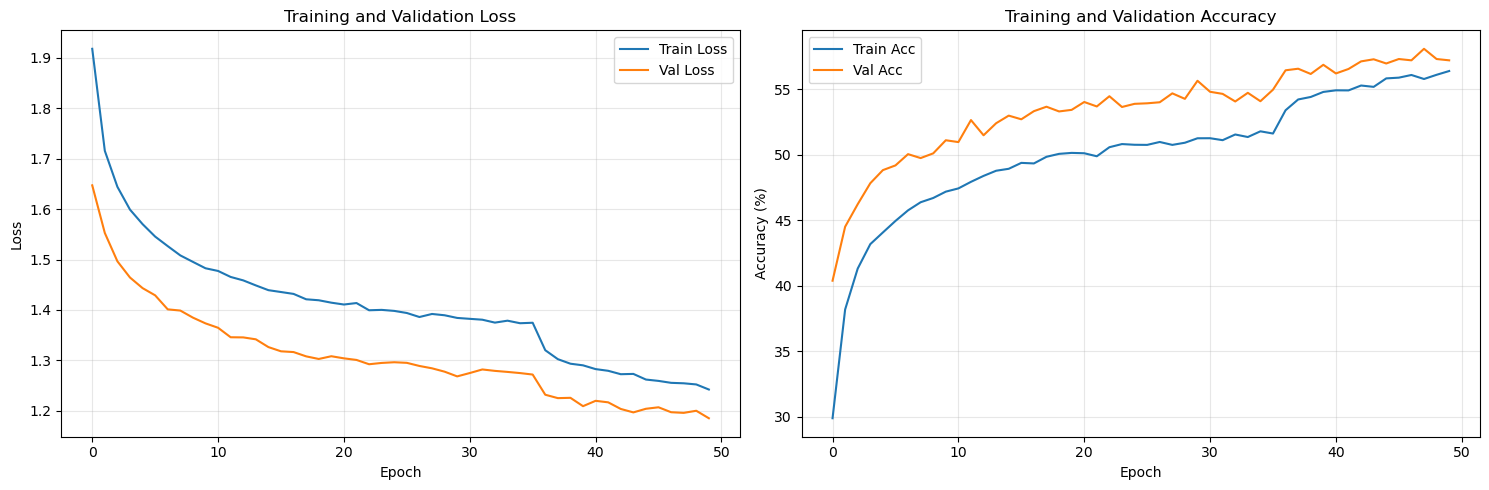
\includegraphics[width=0.85\linewidth]{images/part1_linechart3.png}
    \caption{Training and validation accuracy/loss curves of the PyTorch MLP on CIFAR-10 across 50 epochs.}
    \label{fig:cifar-curves}
\end{figure}

The model's performance is limited by the dense architecture's inability to exploit spatial structure in images. Compared to convolutional neural networks, MLPs require significantly more parameters (over 2 million) to capture spatial correlations, leading to slower convergence. The lack of translation invariance means the model must learn separate representations for the same object at different positions. Future improvements could include replacing the MLP with convolutional layers or applying more sophisticated data augmentation techniques.

\section{Part II: PyTorch CNN (30 points)}
In the second part of Assignment~2, I implement a convolutional neural network (CNN) architecture using PyTorch to improve image classification performance on CIFAR-10. This section covers two main tasks: implementing the CNN architecture and training procedure (Task~1), and analyzing the model's performance with accuracy and loss curves (Task~2).

\subsection{Task 1: Architecture and Training Procedure}
\paragraph{Model Architecture.} I implement a reduced version of the VGG network architecture for CIFAR-10 classification. The CNN consists of 8 convolutional layers organized into 5 blocks, each followed by max pooling, with batch normalization applied after each convolutional layer. The architecture progressively increases the number of channels while reducing spatial dimensions through pooling operations.

Figure~\ref{fig:cnn-architecture} illustrates the complete network architecture, showing the layer-by-layer structure and connections. The network processes $32 \times 32 \times 3$ CIFAR-10 images through convolutional blocks that extract increasingly complex features, ultimately producing 10-class logits.

\begin{figure}[h]
    \centering
    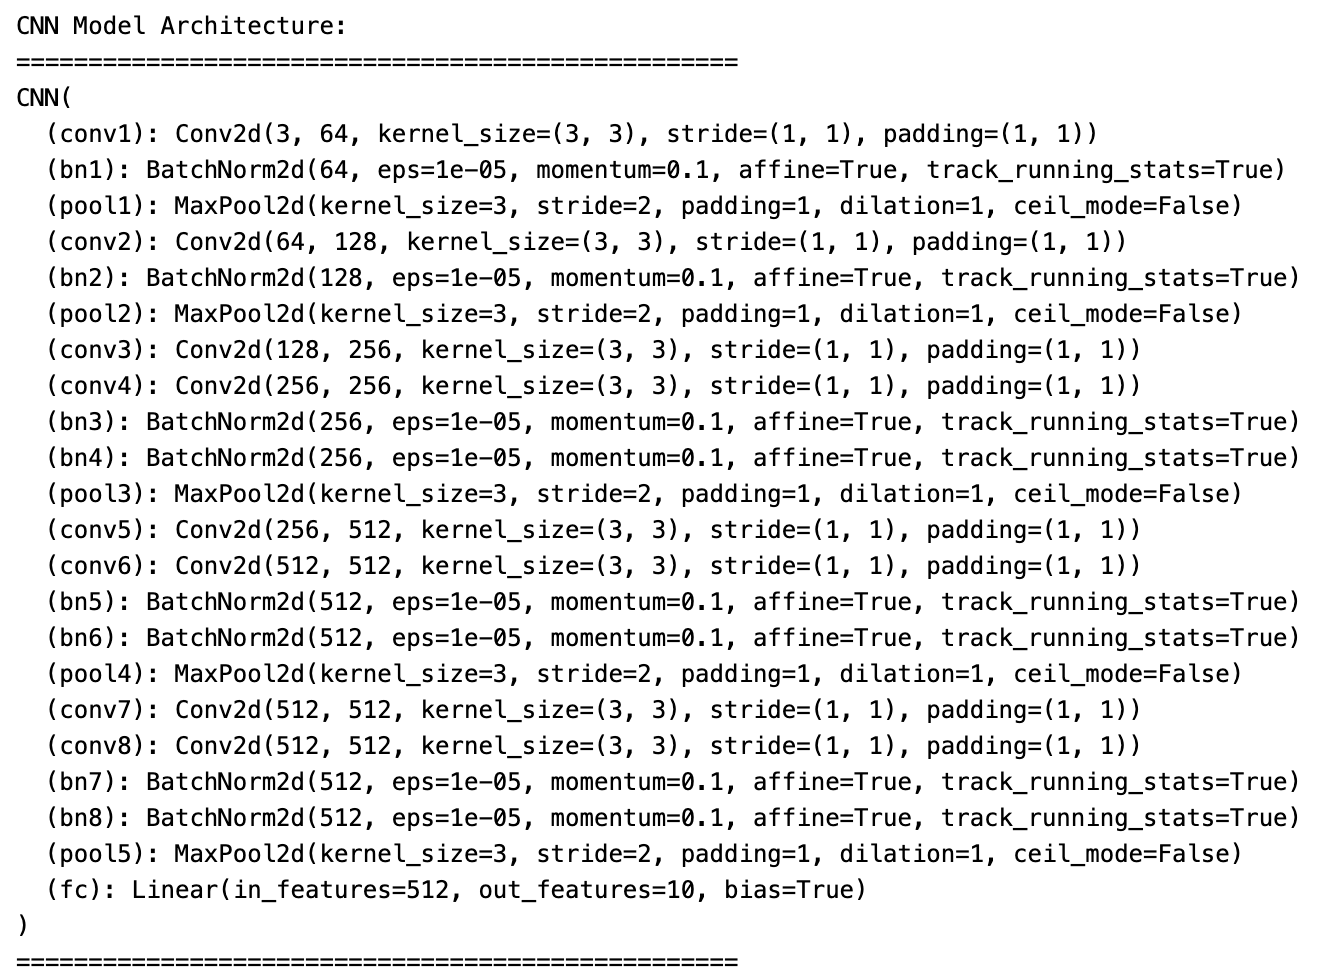
\includegraphics[width=0.9\linewidth]{images/part2_architecture.png}
    \caption{CNN architecture diagram showing the layer structure and connections.}
    \label{fig:cnn-architecture}
\end{figure}

\paragraph{Dimension Evolution During Forward Propagation.} For a batch of size $N$, the tensor dimensions evolve through each layer as follows:

\begin{align*}
\mathbf{x}_0 &\in \mathbb{R}^{N \times 3 \times 32 \times 32} && \text{input images} \\
\mathbf{x}_1 &= \text{ReLU}(\text{BN}(\text{Conv2d}(\mathbf{x}_0))) \in \mathbb{R}^{N \times 64 \times 32 \times 32} && \text{conv1: } 3 \rightarrow 64 \text{ channels} \\
\mathbf{x}_2 &= \text{MaxPool2d}(\mathbf{x}_1) \in \mathbb{R}^{N \times 64 \times 16 \times 16} && \text{pool1: spatial } 32 \rightarrow 16 \\
\mathbf{x}_3 &= \text{ReLU}(\text{BN}(\text{Conv2d}(\mathbf{x}_2))) \in \mathbb{R}^{N \times 128 \times 16 \times 16} && \text{conv2: } 64 \rightarrow 128 \text{ channels} \\
\mathbf{x}_4 &= \text{MaxPool2d}(\mathbf{x}_3) \in \mathbb{R}^{N \times 128 \times 8 \times 8} && \text{pool2: spatial } 16 \rightarrow 8 \\
\mathbf{x}_5 &= \text{ReLU}(\text{BN}(\text{Conv2d}(\mathbf{x}_4))) \in \mathbb{R}^{N \times 256 \times 8 \times 8} && \text{conv3: } 128 \rightarrow 256 \\
\mathbf{x}_6 &= \text{ReLU}(\text{BN}(\text{Conv2d}(\mathbf{x}_5))) \in \mathbb{R}^{N \times 256 \times 8 \times 8} && \text{conv4: } 256 \rightarrow 256 \\
\mathbf{x}_7 &= \text{MaxPool2d}(\mathbf{x}_6) \in \mathbb{R}^{N \times 256 \times 4 \times 4} && \text{pool3: spatial } 8 \rightarrow 4 \\
\mathbf{x}_8 &= \text{ReLU}(\text{BN}(\text{Conv2d}(\mathbf{x}_7))) \in \mathbb{R}^{N \times 512 \times 4 \times 4} && \text{conv5: } 256 \rightarrow 512 \\
\mathbf{x}_9 &= \text{ReLU}(\text{BN}(\text{Conv2d}(\mathbf{x}_8))) \in \mathbb{R}^{N \times 512 \times 4 \times 4} && \text{conv6: } 512 \rightarrow 512 \\
\mathbf{x}_{10} &= \text{MaxPool2d}(\mathbf{x}_9) \in \mathbb{R}^{N \times 512 \times 2 \times 2} && \text{pool4: spatial } 4 \rightarrow 2 \\
\mathbf{x}_{11} &= \text{ReLU}(\text{BN}(\text{Conv2d}(\mathbf{x}_{10}))) \in \mathbb{R}^{N \times 512 \times 2 \times 2} && \text{conv7: } 512 \rightarrow 512 \\
\mathbf{x}_{12} &= \text{ReLU}(\text{BN}(\text{Conv2d}(\mathbf{x}_{11}))) \in \mathbb{R}^{N \times 512 \times 2 \times 2} && \text{conv8: } 512 \rightarrow 512 \\
\mathbf{x}_{13} &= \text{MaxPool2d}(\mathbf{x}_{12}) \in \mathbb{R}^{N \times 512 \times 1 \times 1} && \text{pool5: spatial } 2 \rightarrow 1 \\
\mathbf{x}_{14} &= \text{Flatten}(\mathbf{x}_{13}) \in \mathbb{R}^{N \times 512} && \text{flattened} \\
\mathbf{y} &= \text{Linear}(\mathbf{x}_{14}) \in \mathbb{R}^{N \times 10} && \text{output logits}
\end{align*}

The convolutional layers use $3 \times 3$ kernels with padding 1 to preserve spatial dimensions, and max pooling uses $3 \times 3$ kernels with stride 2 and padding 1, reducing spatial dimensions by half. Each convolutional layer has parameters: weights $\mathbf{W} \in \mathbb{R}^{C_{\text{out}} \times C_{\text{in}} \times 3 \times 3}$ and bias $\mathbf{b} \in \mathbb{R}^{C_{\text{out}}}$, where $C_{\text{in}}$ and $C_{\text{out}}$ are input and output channel numbers. Batch normalization layers add $2 \times C$ parameters per channel. The total number of parameters is approximately 9.4 million, which is more than the MLP but achieves much better performance due to parameter sharing and translation invariance.

\paragraph{Training Procedure.} The model is trained on CIFAR-10 using the Adam optimizer with learning rate $1 \times 10^{-4}$, batch size 32, and mini-batch gradient descent. Data augmentation includes random horizontal flip and random crop with 4-pixel padding, followed by normalization. 

Initially, training for 5000 epochs (as specified in the default configuration) was attempted, but this led to overfitting and required over 12 hours of training time; after that I tried to train for 5000 steps, which led to underoverfitting. Therefore, I choose to train for 500 epochs with early stopping enabled. The early stopping mechanism uses patience 5 and minimum delta 0.05 to prevent overfitting. Model checkpoints are saved when validation accuracy improves, and the best model is used for final evaluation. This approach balances training efficiency with model performance, achieving good generalization without excessive training time.

\subsection{Task 2: Performance Analysis}
\paragraph{Results and Analysis.} Table~\ref{tab:cnn-results} presents the final performance metrics. The CNN achieves 86.60\% test accuracy, significantly outperforming the MLP (58.04\%) by 28.56 percentage points. This substantial improvement demonstrates the effectiveness of convolutional layers in capturing spatial features and translation-invariant patterns in images.

\begin{table}[h]
    \centering
    \caption{CIFAR-10 performance of the PyTorch CNN (best checkpoint with early stopping).}
    \label{tab:cnn-results}
    \begin{tabular}{@{}lcc@{}}
        \toprule
        Split & Accuracy (\%) & Loss \\
        \midrule
        Training & 98.97 & 0.0315 \\
        Test & 86.60 & -- \\
        \bottomrule
    \end{tabular}
\end{table}

Figure~\ref{fig:cnn-curves} shows the training and test accuracy/loss curves. The training accuracy reaches 98.97\%, while test accuracy plateaus around 86.60\%, indicating a generalization gap of approximately 12.37\%. This gap is expected and acceptable, as the model learns discriminative features without severe overfitting thanks to batch normalization and early stopping. The loss curves show smooth convergence, with training loss decreasing steadily to 0.0315.

\begin{figure}[h]
    \centering
    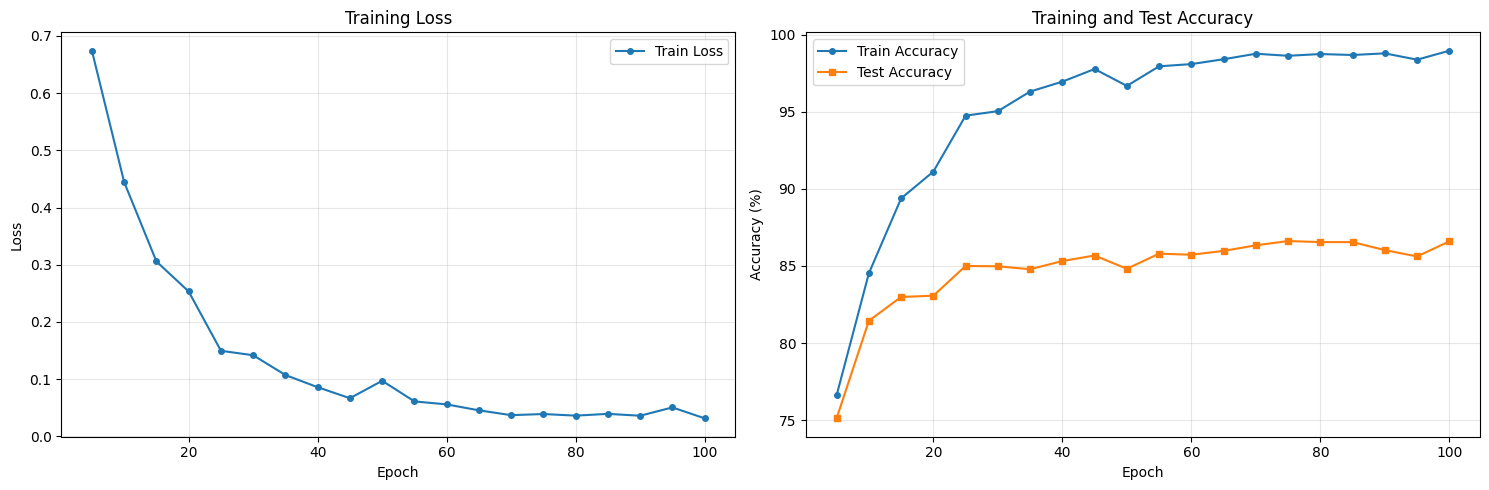
\includegraphics[width=0.85\linewidth]{images/part2_linechart1.png}
    \caption{Training and test accuracy/loss curves of the PyTorch CNN on CIFAR-10.}
    \label{fig:cnn-curves}
\end{figure}

The CNN's superior performance compared to the MLP can be attributed to several key advantages: (1) \textbf{Parameter sharing}: Convolutional filters are shared across spatial locations, dramatically reducing the number of parameters while maintaining model capacity. (2) \textbf{Translation invariance}: The model can recognize objects regardless of their position in the image, a crucial property for image classification. (3) \textbf{Spatial feature extraction}: Convolutional layers naturally capture local patterns (edges, textures) that are then combined into higher-level features (shapes, objects). (4) \textbf{Efficient computation}: The reduced parameter count and efficient convolution operations enable faster training and better generalization.

The architecture successfully balances model capacity and generalization, achieving strong performance on CIFAR-10 while maintaining reasonable training time. The early stopping mechanism prevents overfitting, ensuring the model generalizes well to unseen test data.

\section{Part III: PyTorch RNN (40 points)}
In the third part of Assignment~2, I implement a vanilla recurrent neural network (RNN) from scratch using PyTorch to predict the last digit of palindromes. This section covers two main tasks: implementing the vanilla RNN architecture and training procedure (Task~1), and analyzing the model's performance across different palindrome lengths (Task~2).

\subsection{Task 1: Architecture and Training Procedure}
\paragraph{Model Architecture.} I implement a vanilla RNN from scratch without using PyTorch's built-in \texttt{torch.nn.RNN} or \texttt{torch.nn.LSTM} modules. The RNN is designed to process sequences of digits and predict the last digit of a palindrome given the preceding digits.

The RNN follows the standard recurrence equations:
\begin{align*}
\mathbf{h}^{(t)} &= \tanh(\mathbf{x}^{(t)} \mathbf{W}_{xh} + \mathbf{h}^{(t-1)} \mathbf{W}_{hh} + \mathbf{b}_h) \\
\mathbf{o}^{(t)} &= \mathbf{h}^{(t)} \mathbf{W}_{hy} + \mathbf{b}_y \\
\hat{\mathbf{y}}^{(t)} &= \text{softmax}(\mathbf{o}^{(t)})
\end{align*}
where $\mathbf{x}^{(t)} \in \mathbb{R}^{N \times 1}$ is the input at time step $t$, $\mathbf{h}^{(t)} \in \mathbb{R}^{N \times H}$ is the hidden state, $\mathbf{o}^{(t)} \in \mathbb{R}^{N \times 10}$ are the output logits, and $\hat{\mathbf{y}}^{(t)} \in \mathbb{R}^{N \times 10}$ are the predicted probabilities. The initial hidden state $\mathbf{h}^{(0)}$ is initialized as a zero vector.

\paragraph{Dimension Evolution During Forward Propagation.} For a batch of size $N$ and sequence length $T$, the tensor dimensions evolve through each time step as follows:

\begin{align*}
\mathbf{x}^{(t)} &\in \mathbb{R}^{N \times 1} && \text{input digit at time } t \\
\mathbf{h}^{(0)} &= \mathbf{0} \in \mathbb{R}^{N \times H} && \text{initial hidden state (zeros)} \\
\mathbf{h}^{(t)} &= \tanh(\mathbf{x}^{(t)} \mathbf{W}_{xh} + \mathbf{h}^{(t-1)} \mathbf{W}_{hh} + \mathbf{b}_h) \in \mathbb{R}^{N \times H} && \mathbf{W}_{xh} \in \mathbb{R}^{1 \times H}, \mathbf{W}_{hh} \in \mathbb{R}^{H \times H}, \mathbf{b}_h \in \mathbb{R}^{H} \\
\mathbf{o}^{(T)} &= \mathbf{h}^{(T)} \mathbf{W}_{hy} + \mathbf{b}_y \in \mathbb{R}^{N \times 10} && \mathbf{W}_{hy} \in \mathbb{R}^{H \times 10}, \mathbf{b}_y \in \mathbb{R}^{10} \\
\hat{\mathbf{y}}^{(T)} &= \text{softmax}(\mathbf{o}^{(T)}) \in \mathbb{R}^{N \times 10} && \text{predicted probabilities}
\end{align*}

The loss is computed only over the last time step $T$: $\mathcal{L} = -\sum_{k=1}^{10} y_k \log(\hat{y}_k^{(T)})$, where $\mathbf{y}$ is the one-hot encoded target (the last digit of the palindrome).

\paragraph{Training Procedure.} The model is trained on the \texttt{PalindromeDataset}, which generates random palindromes of specified length. Each palindrome is split into input sequence (first $T-1$ digits) and target (last digit). Training uses RMSprop optimizer with learning rate $1 \times 10^{-3}$, batch size 128, and 500 training steps. Gradient clipping with max norm 10.0 is applied to prevent exploding gradients, which is crucial for RNN training stability.

\subsection{Task 2: Performance Analysis Across Palindrome Lengths}
\paragraph{Experimental Setup.} To analyze how RNN performance varies with sequence length, I train separate models for palindrome lengths ranging from 5 to 50 (increments of 5). For each length, a fresh RNN is trained for 500 steps, and evaluation accuracy is measured on 50 batches of test data. This experiment reveals the RNN's memory limitations as sequence length increases.

\paragraph{Results and Analysis.} Table~\ref{tab:rnn-results} presents the evaluation accuracy for different palindrome lengths. The RNN achieves near-perfect accuracy (99.44\%) for length 5, demonstrating excellent performance on short sequences. However, accuracy degrades significantly as sequence length increases: 87.20\% for length 10, 86.71\% for length 15, and drops to 47.40\% for length 20. For lengths 25 and above, accuracy approaches random chance (approximately 10\%), indicating that the RNN has effectively lost the ability to maintain information about early digits in the sequence.

\begin{table}[h]
    \centering
    \caption{RNN evaluation accuracy across different palindrome lengths.}
    \label{tab:rnn-results}
    \begin{tabular}{@{}lcc@{}}
        \toprule
        Length & Train Acc (\%) & Eval Acc (\%) \\
        \midrule
        5 & 91.41 & 99.44 \\
        10 & 89.84 & 87.20 \\
        15 & 86.72 & 86.71 \\
        20 & 30.47 & 47.40 \\
        25 & 6.25 & 9.79 \\
        30 & 7.81 & 9.72 \\
        35 & 8.59 & 10.03 \\
        40 & 7.81 & 9.93 \\
        45 & 5.47 & 10.34 \\
        50 & 10.94 & 10.29 \\
        \bottomrule
    \end{tabular}
\end{table}

Figure~\ref{fig:rnn-accuracy} visualizes the relationship between palindrome length and evaluation accuracy. The plot clearly shows a sharp decline in performance as sequence length increases beyond 15, confirming the vanishing gradient problem inherent in vanilla RNNs. The model successfully learns short-range dependencies (lengths 5-15) but fails to maintain information over longer sequences.

\begin{figure}[h]
    \centering
    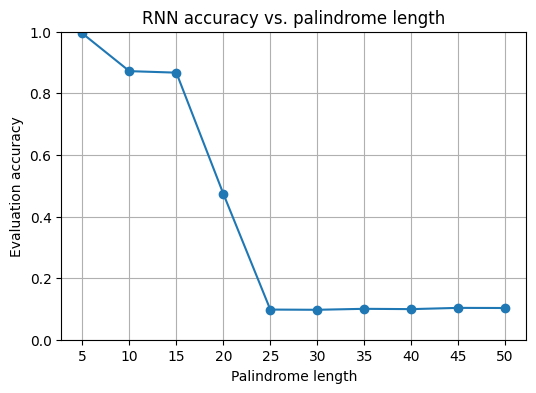
\includegraphics[width=0.75\linewidth]{images/part3_accuracy-line.png}
    \caption{Evaluation accuracy vs. palindrome length for the vanilla RNN.}
    \label{fig:rnn-accuracy}
\end{figure}

\paragraph{Detailed Analysis.} The experimental results reveal key insights about vanilla RNNs: (1) \textbf{Short-range dependencies:} The RNN excels at learning patterns in short sequences (lengths 5-15), achieving accuracy above 86\%, demonstrating effective capture of local patterns. (2) \textbf{Memory limitations:} The dramatic performance drop at length 20 (47.40\%) and near-random performance for lengths 25+ (approximately 10\%) reveals the vanishing gradient problem. As gradients propagate backward through time, they diminish exponentially, making it difficult to learn long-range dependencies. (3) \textbf{Task complexity:} Predicting the last digit of a palindrome requires remembering the first digit throughout the entire sequence, which is particularly challenging for vanilla RNNs.

\end{document}

